% !TeX encoding = UTF-8
% !TeX spellcheck = de_DE

%% Dies gibt Warnungen aus, sollten veraltete LaTeX-Befehle verwendet werden
\RequirePackage[l2tabu, orthodox]{nag}

\documentclass[utf8,biblatex]{lni}
\bibliography{lni-paper-example-de}

%% Schöne Tabellen mittels \toprule, \midrule, \bottomrule
\usepackage{booktabs}

%% Zu Demonstrationszwecken
\usepackage[math]{blindtext}
\usepackage{mwe}

%% BibLaTeX-Sonderkonfiguration,
%% falls man schnell eine existierende Bibliographie wiederverwenden will, aber nicht die .bib-Datei händisch anpassen möchte.
%% Bitte \iffalse und \fi entfernen, dann ist diese Konfiguration aktiviert.

\iffalse
\AtEveryBibitem{%
  \ifentrytype{article}{%
  }{%
    \clearfield{doi}%
    \clearfield{issn}%
    \clearfield{url}%
    \clearfield{urldate}%
  }%
  \ifentrytype{inproceedings}{%
  }{%
    \clearfield{doi}%
    \clearfield{issn}%
    \clearfield{url}%
    \clearfield{urldate}%
  }%
}
\fi

\begin{document}
%%% Mehrere Autoren werden durch \and voneinander getrennt.
%%% Die Fußnote enthält die Adresse sowie eine E-Mail-Adresse.
%%% Das optionale Argument (sofern angegeben) wird für die Kopfzeile verwendet.
\title[Ein Kurztitel]{Windows Subsystem for Linux}
%%%\subtitle{Untertitel / Subtitle} % falls benötigt
\author[Marius Rusu \and Julia Sommer]
{Marius Rusu\footnote{Ludwig-Maximilian-Universität München, Fakultät für Informatik, Oettingenstraße 67, 80538 München, Deutschland \email{rusu.marius97@gmail.com}} \and
 Julia Sommer\footnote{Technische Universität München, Fakultät für Informatik, Boltzmanstraße 3, 85748 Garching, Deutschland \email{sommerjulia99@gmail.com}}}
\startpage{11} % Beginn der Seitenzählung für diesen Beitrag
\editor{Herausgeber et al.}    % Namen der Herausgeber
\booktitle{Name-der-Konferenz} % Name des Tagungsband
\year{2017}
%%%\lnidoi{18.18420/provided-by-editor-02} % Falls bekannt
\maketitle

\begin{abstract}
Die \LaTeX-Klasse \texttt{lni} setzt die Layout-Vorgaben für Beiträge in LNI Konferenzbänden um.
Dieses Dokument beschreibt ihre Verwendung und ist ein Beispiel für die entsprechende Darstellung.
Der Abstract ist ein kurzer Überblick über die Arbeit der zwischen 70 und 150 Wörtern lang sein und das Wichtigste enthalten sollte.
Die Formatierung erfolgt automatisch innerhalb des abstract-Bereichs.
\end{abstract}

\begin{keywords}
LNI Guidelines \and \LaTeX Vorlage
\end{keywords}
\section{Microsoft's reasons for WSL}
\section{WSL - What is it?}


\subsection{General Concept}
"Windows Subsystem for Linux is a collection of [user mode and kernel mode] components that enable native Linux ELF64 binaries to run on Windows."\footnote{} User mode applications are low privileged and depend on system calls to operate on kernel mode. Only in kernel mode low level operations directly handled by the operating system can be executed. In WSL we have the bash.exe running in user mode and initiating the Linux Instance. Further this instance submits, if necessary, native Linux system calls to be executed on a Linux Kernel. However, by virtualizing a Linux Kernel interface those system calls can be executed directly on the Windows Kernel. This virtualization is done by the LXCore/LXSS running in kernel mode.\footnote{ https://blogs.msdn.microsoft.com/wsl/2016/04/22/windows-subsystem-for-linux-overview/, 18.04.2018 19:32 Uhr}

\subsection{Basic Architecture}

\begin{comment}

(Windows Subsystem for Linux \glqq is primarily comprised of: 
\begin{enumerate}
    \item User mode session manager service [...]
    \item Pico provider drivers [...]
    \item Pico processes [...] \grqq\footnote{}
\end{enumerate})

\end{comment}

Windows Subsystem for Linux is primarily comprised of: 
\begin{enumerate}
    \item LX Session Manager
    \item LXCore/LXSS
    \item Pico processes\footnote{}
\end{enumerate}

\begin{figure}
  \centering
  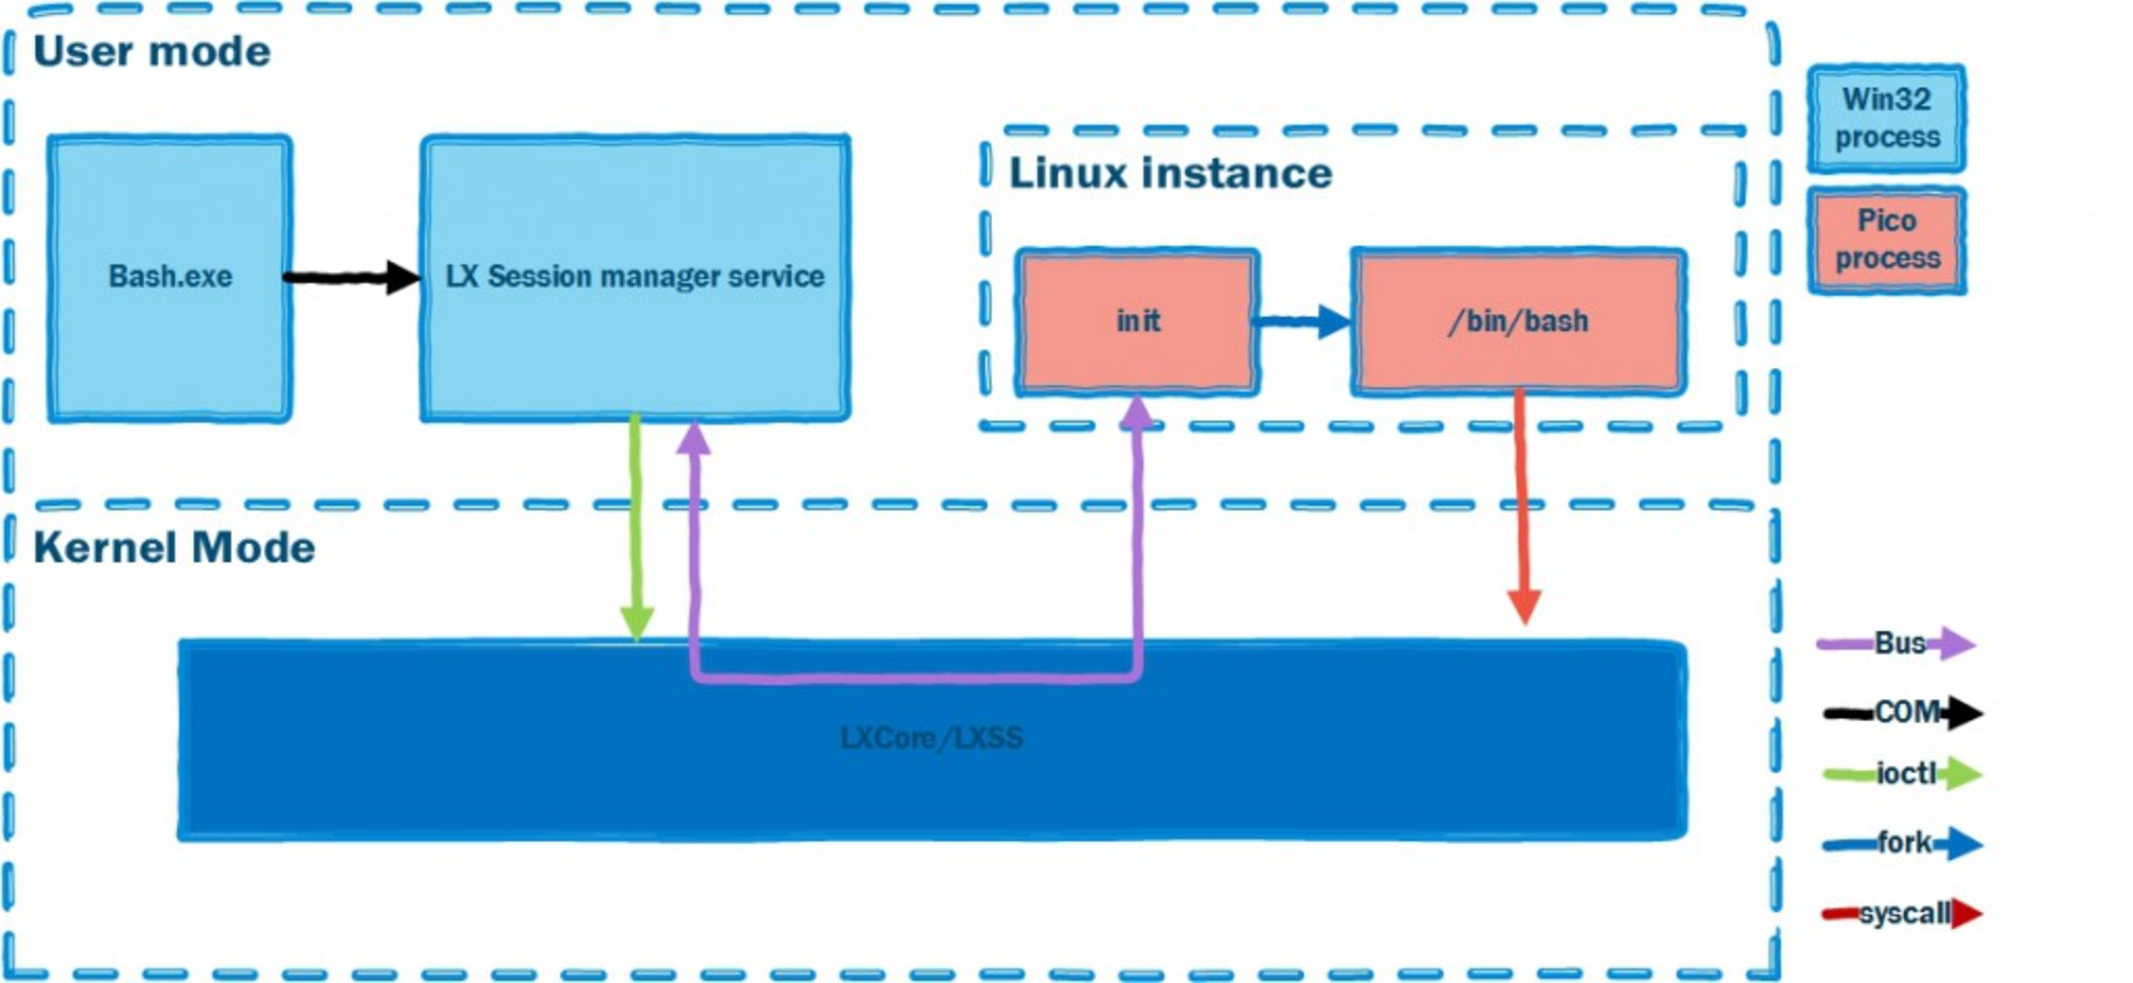
\includegraphics[width=1\textwidth]{WSL Architecture.pdf}
  \caption{Components of WSL}
  \label{img:architecture}
\end{figure}


As depicted in the image above, the user initiates the Windows Subsystem for Linux by launching the bash.exe on Windows. This application then calls the LXCore/LXSS (green arrow) which is a "[...] driver behaving like a Linux Kernel and working in coordination with the Windows Kernel. [The Driver] would then spin up a native Linux process [being] /bin/bash (purple arrow)."\footnote{https://blogs.msdn.microsoft.com/wsl/2016/05/23/pico-process-overview/} All other Linux processes run under /bin/bash in the so called Linux Instance that "[...] you can think of as [...] a container or a virtualized operating system environment." \footnote{https://blogs.msdn.microsoft.com/wsl/2016/05/23/pico-process-overview/}

\glqq By wrapping unmodified Linux binaries into Pico processes we enable Linux system calls to be directed into the Windows kernel.\grqq \footnote{} A Pico process itself is an empty process, as far as the Windows kernel is concerned and therefore cannot be handled by the Windows kernel but instead is redirected to the LXCore/LXSS (red arrow).\footnote{https://blogs.msdn.microsoft.com/wsl/2016/05/23/pico-process-overview/}
That's why it's safe to say, that \glqq Pico processes and drivers [LXCore/LXSS] provide the foundation for the Windows Subsystem for Linux [...]. \grqq \footnote

\begin{comment}

As mentioned, those system calls are native Linux system calls. Therefore the LXCore/LXSS being an emulation of the Linux Kernel\footnote{https://blogs.msdn.microsoft.com/wsl/2016/04/22/windows-subsystem-for-linux-overview/} map those system calls to an equivalent Windows system call to run on the Windows Kernel. However this is not always possible e.g. the operation fork() does not have a Windows equivalent. In that case the Windows Kernel has to handle the system call directly and satisfy its needs.

\end{comment}

\subsection{Implementation of its components}

Despite the fact that there is little known about the implementation of the Windows subsystem for Linux, we are trying to present the known facts as far as possible.

\glqq The pico process concept originated in MSR [Microsoft Research] as part of the Drawbridge project. A goal of this project was to implement a lightweight way to run an application in an isolated environment, with the application’s OS dependencies decoupled from the underlying host OS\glqq \footnote{https://blogs.msdn.microsoft.com/wsl/2016/05/23/pico-process-overview/} This was achieved, not by a Virtual machine, which would be too resource consuming but by \glqq run[ning] the target application and OS entirely within the user-mode address space of a single process on the host OS. \glqq \footnote{https://blogs.msdn.microsoft.com/wsl/2016/05/23/pico-process-overview/} \glqq The Drawbridge pico process is a lightweight, secure isolation container. It is built from an OS process address space, but with all traditional OS services removed. [...] All ABI [Application binary interface] calls are serviced by the security monitor, which plays a role similar to the hypervisor or VM monitor in traditional hardware VM designs.\glqq \footnote{https://www.microsoft.com/en-us/research/project/drawbridge/?from=http\%3A\%2F\%2Fresearch.microsoft.com\%2Fen-us\%2Fproject s\%2Fdrawbridge\%2F}

In case of Windows subsystem for Linux this is exactly the point where pico processes are redirected to the LXCore/LXSS. \glqq The drivers do not contain code from the Linux kernel but are instead a clean room implementation of Linux-compatible kernel interfaces. [..] Where possible, lxcore.sys translates the Linux syscall to the equivalent Windows NT call which in turn does the heavy lifting. Where there is no reasonable mapping the Windows kernel mode driver must service the request directly.\glqq \footnote{} Since the Windows Kernel was originally designed to support multiple operating systems, Microsoft had to \glqq [dust] [...] of old functionality, [enhance] it for performance and correctness and it was able to go right away.\glqq \footnote{https://blogs.msdn.microsoft.com/wsl/2016/05/23/pico-process-overview/} Those changes in the Windows kernel enable it to execute even foreign operations like fork(). Windows applications however do not have access to those specific Linux system calls. \footnote{}

\glqq The File system support in WSL was designed to meet two goals:
\begin{enumerate}
    \item Provide an environment that supports the full fidelity of Linux file systems
    \item Allow interoperability with drives and files in Windows
\end{enumerate}\footnote{https://blogs.msdn.microsoft.com/wsl/2016/04/22/windows-subsystem-for-linux-overview/}

\glqq VolFs is a file system that provides full support for Linux file system features, including Linux permissions that can be modified through operations such as chmod and chroot [etc].\glqq \footnote{https://blogs.msdn.microsoft.com/wsl/2016/04/22/windows-subsystem-for-linux-overview/} Due to the fact that VolFs file system is not able to interoperate with Windows, a second file system named DriveFs is implemented. \glqq All fixed Windows volumes are mounted under /mnt [...] where users can access all Windows files.\glqq \footnote{https://blogs.msdn.microsoft.com/wsl/2016/04/22/windows-subsystem-for-linux-overview/} To make this possible the DriveFs file system meets Windows requirements such as legal file names and Windows security but looses some of the Linux features.

\section{Alternatives to Windows Subsystem for Linux}
\subsection{Classical approach to virtualization}

\subsection{Virtualization via Virtual Machine}

\begin{figure}
  \centering
  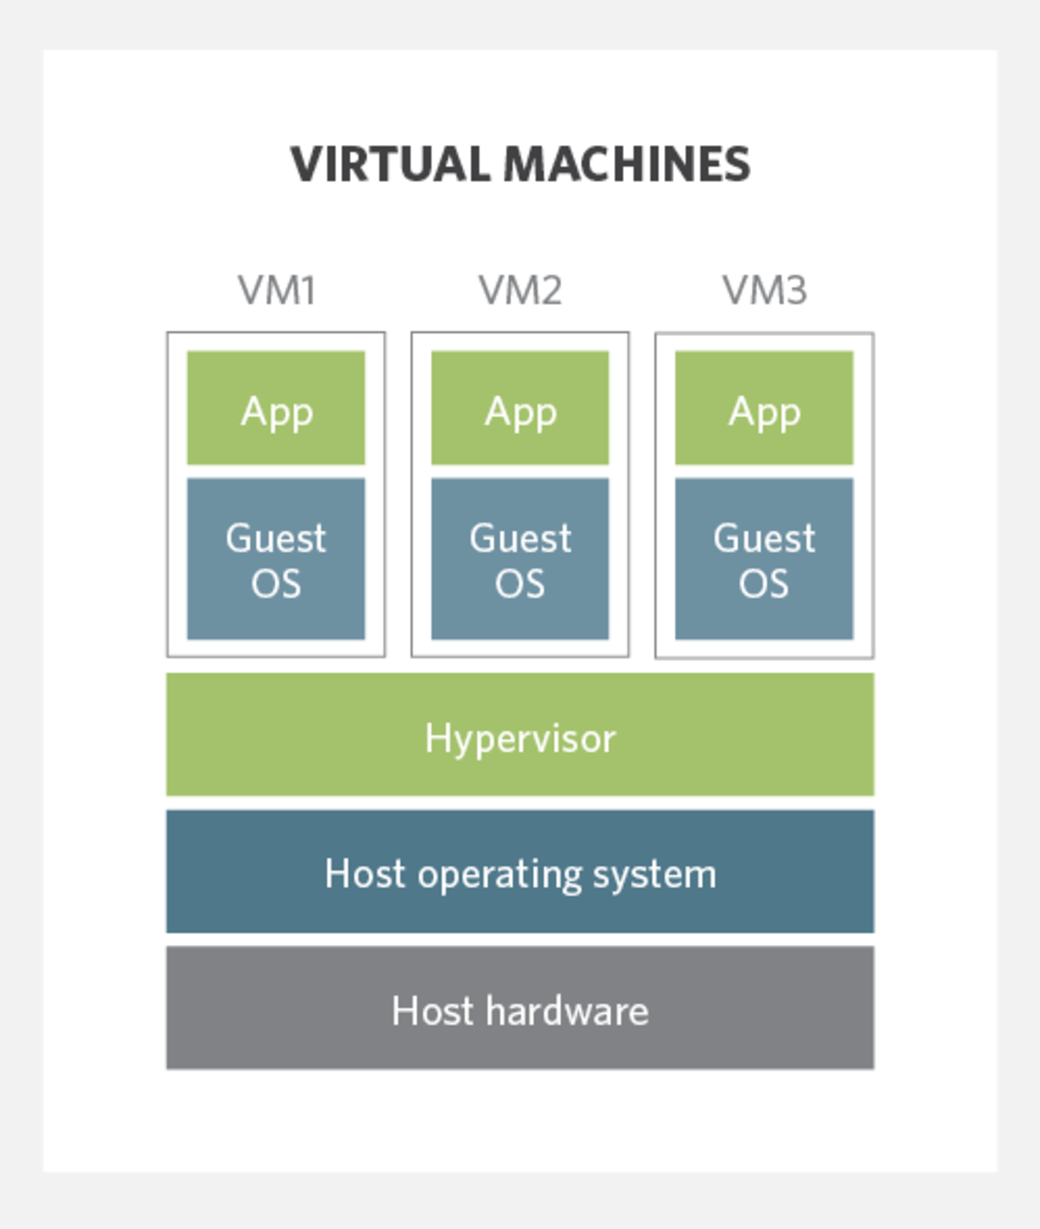
\includegraphics[width=0.5\textwidth]{VM.pdf}
  \caption{Virtual Machine Overview}
  \label{img:vm}
\end{figure}

\glqq The virtual machine concept allows the same computer to be shared as if it were several. IBM defined the virtual machine as a fully protected and isolated copy of the underlying physical machine’s hardware. \glqq\footnote{R. Rose, \glqq Survey of System Virtualization Techniques \glqq https://ir.library.oregonstate.edu/concern/parent/t148fh24b/file_sets/0r967383v} 
Therefore it is possible to run different applications on different operating systems at the same time on the same hardware as depicted in the image above. \glqq The VMM [Virtual Machine Monitor] is the software component that hosts guest virtual machines.\glqq \footnote{https://ir.library.oregonstate.edu/concern/parent/t148fh24b/file_sets/0r967383v}
According to Prof. Dr. Kranzmüller and Dr. Danciu the Virtual Machine Monitor is firstly responsible for coordinating the access of the guest operation systems on the host's hardware and secondly for handling traps. Traps are created when a guest operating system is trying to execute a privileged operation. In that case, the Virtual Machine Monitor emulates its function in order to be executed on the host operating system. \footnote{Skript!}

\subsection{Virtualization via Container}

\begin{figure}
  \centering
  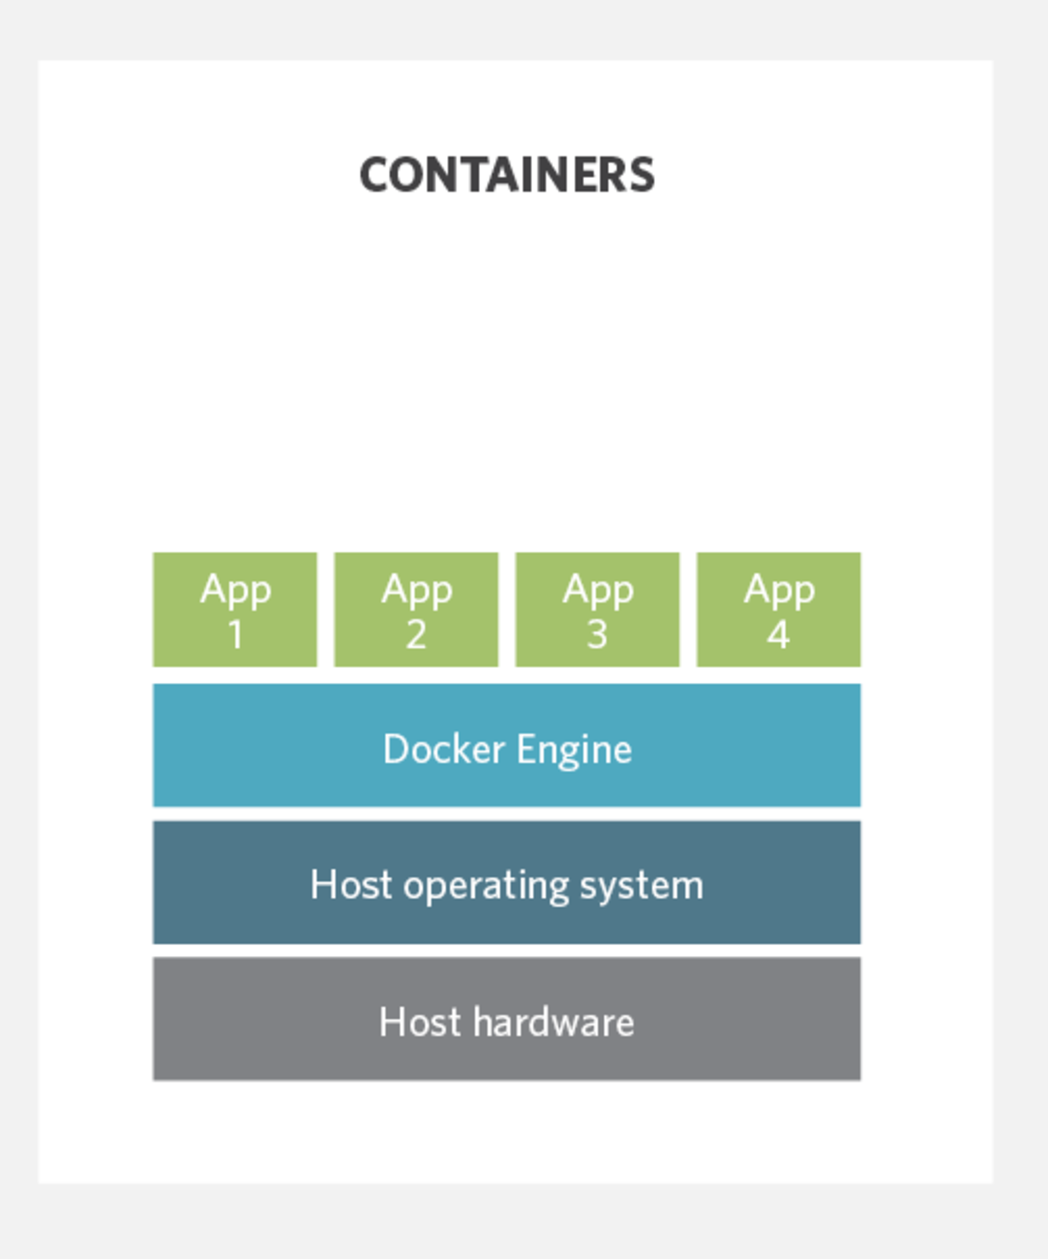
\includegraphics[width=0.5\textwidth]{Container.pdf}
  \caption{Container Overview}
  \label{img:container}
\end{figure}

Instead of a Virtual Machine Monitor there is a container engine, also called Docker engine running on top on the host operating system which can be seen in the image above. \glqq A container engine is a managed environment for deploying containerized applications. The container engine allocates cores and memory to containers [and] enforces spatial isolation and security [...] \glqq \footnote{https://insights.sei.cmu.edu/sei_blog/2017/09/virtualization-via-containers.html}


Dieses Template ist wie folgt gegliedert:
\Cref{sec:demos} zeigt Demonstrationen der LNI-Verlage.
\Cref{sec:lniconformance} zeigt die Einhaltung der Richtlinien durch einfachen Text.

\section{Demonstrationen}
\label{sec:demos}
Das Symbol für Potenzmengen ($\powerset$) wird korrekt angezeigt.
Es ist kein Weierstraß-p ($\wp$) mehr.

Spitze Klammen können direkt eingegeben werden: <test />

Hier eine kleine Demonstration von \href{https://www.ctan.org/pkg/microtype}{microtype}:
\blindtext

\section{Demonstration der Einhaltung der Richtlinien}
\label{sec:lniconformance}

\subsection{Literaturverzeichnis}
Der letzte Abschnitt zeigt ein beispielhaftes Literaturverzeichnis für Bücher mit einem Autor \cite{Ez10} und zwei AutorInnen \cite{AB00}, einem Beitrag in Proceedings mit drei AutorInnen \cite{ABC01}, einem Beitrag in einem LNI Band mit mehr als drei AutorInnen \cite{Az09}, zwei Bücher mit den jeweils selben vier AutorInnen im selben Erscheinungsjahr \cite{Wa14} und \cite{Wa14b}, ein Journal \cite{Gl06}, eine Website \cite{GI14} bzw.\ anderweitige Literatur ohne konkrete AutorInnenschaft \cite{XX14}.
Es wird biblatex verwendet, da es UTF8 sauber unterstützt und \href{https://github.com/gi-ev/LNI/issues/5}{im Gegensatz zu lni.bst} keine Fehler beim bibtexen auftreten.

Referenzen sollten nicht direkt als Subjekt eingebunden werden, sondern immer nur durch Authorenanganben:
Beispiel: \Citet{AB00} geben ein Beispiel, aber auch \citet{Az09}.
Hinweis: Großes C bei \texttt{Citet}, wenn es am Satzanfang steht. Dies ist analog zu \texttt{Cref}.

Formatierung und Abkürzungen werden für die Referenzen \texttt{book}, \texttt{inbook}, \texttt{proceedings}, \texttt{inproceedings}, \texttt{article}, \texttt{online} und \texttt{misc} automatisch vorgenommen.
Mögliche Felder für Referenzen können der Beispieldatei \texttt{lni-paper-example-de.bib} entnommen werden.
Andere Referenzen sowie Felder müssen allenfalls nachträglich angepasst werden.

\subsection{Abbildungen}
\Cref{fig:demo} zeigt eine Abbildung.

\begin{figure}
  \centering
  \includegraphics[width=.8\textwidth]{example-image}
  \caption{Demographik}
  \label{fig:demo}
\end{figure}

\subsection{Tabellen}
\Cref{tab:demo} zeigt eine Tabelle.

\begin{table}
\centering
\begin{tabular}{lll}
\toprule
Überschriftsebenen & Beispiel & Schriftgröße und -art \\
\midrule
Titel (linksbündig) & Der Titel \ldots & 14 pt, Fett\\
Überschrift 1 & 1 Einleitung & 12 pt, Fett\\
Überschrift 2 & 2.1 Titel & 10 pt, Fett\\
\bottomrule
\end{tabular}
\caption{Die Überschriftsarten}
\label{tab:demo}
\end{table}

\subsection{Programmcode}
Die LNI-Formatvorlage verlangt die Einrückung von Listings vom linken Rand.
In der \texttt{lni}-Dokumentenklasse ist dies für die \texttt{verbatim}-Umgebung realisiert.

\begin{verbatim}
public class Hello {
    public static void main (String[] args) {
        System.out.println("Hello World!");
    }
}
\end{verbatim}

Alternativ kann auch die \texttt{lstlisting}-Umgebung verwendet werden.

\Cref{L1} zeigt uns ein Beispiel, das mit Hilfe der \texttt{lstlisting}-Umgebung realisiert ist.

\begin{lstlisting}[caption={Beschreibung}, label=L1]
public class Hello {
    public static void main (String[] args) {
        System.out.println("Hello World!");
    }
}
\end{lstlisting}

\subsection{Formeln und Gleichungen}

Die korrekte Einrückung und Nummerierung für Formeln ist bei den Umgebungen \texttt{equation} und \texttt{eqnarray} gewährleistet.

\begin{equation}
  1=4-3
\end{equation}
und
\begin{eqnarray}
  2=7-5\\
  3=2-1
\end{eqnarray}

%% \bibliography{lni-paper-example-de.tex} ist hier nicht erlaubt: biblatex erwartet dies bei der Preambel
%% Starten Sie "biber paper", um eine Biliographie zu erzeugen.
\printbibliography

\end{document}
